\section*{Цель работы}

\begin{enumerate}
    \item Моделирование и исследование работы мультивибратора в LTspice.
\end{enumerate}



\section*{Мультивибратор на транзисторах}

Модель транзистора - 2N3904. Соьерем схему как на рисунке \ref{fig:мультивибр_транзисторы_схема} 
Значения сопротивления резисторов, а также напряжение питания в 
соответствии с вариантом. Значение емкостей конденсаторов рассчитаем по формуле
\begin{equation*}
    T=0.7(R_3C_2+R_2C_1)=0.7C(R_3+R_2)
\end{equation*}
так, чтобы период генерируемого сигнала соответствовал $T=1$ c.:
\begin{equation*}
    C=\frac{T}{0.7(R_3+R_2)}=\frac{1}{12000 * 7}\approx 1.19\cdot10^{-5}\ \text{Ф}=11.9\ \text{мкФ}.
\end{equation*}

Осцилограммы напряжений с баз и коллекторов транзисторов
можно увидеть на рисунке \ref{fig:Q12}. Схема успешно генерирует колебания. Как видно, период колебаний
составляет около секунды, что сходится с заданным в исходных данных.

Скважность - это отношение периода повторения к длительности импульса
\begin{equation*}
    Q=\frac{T}{t}=\frac{1}{0.7R_2C}\approx 2.00.
\end{equation*}

\begin{figure}[H]
    \centering
    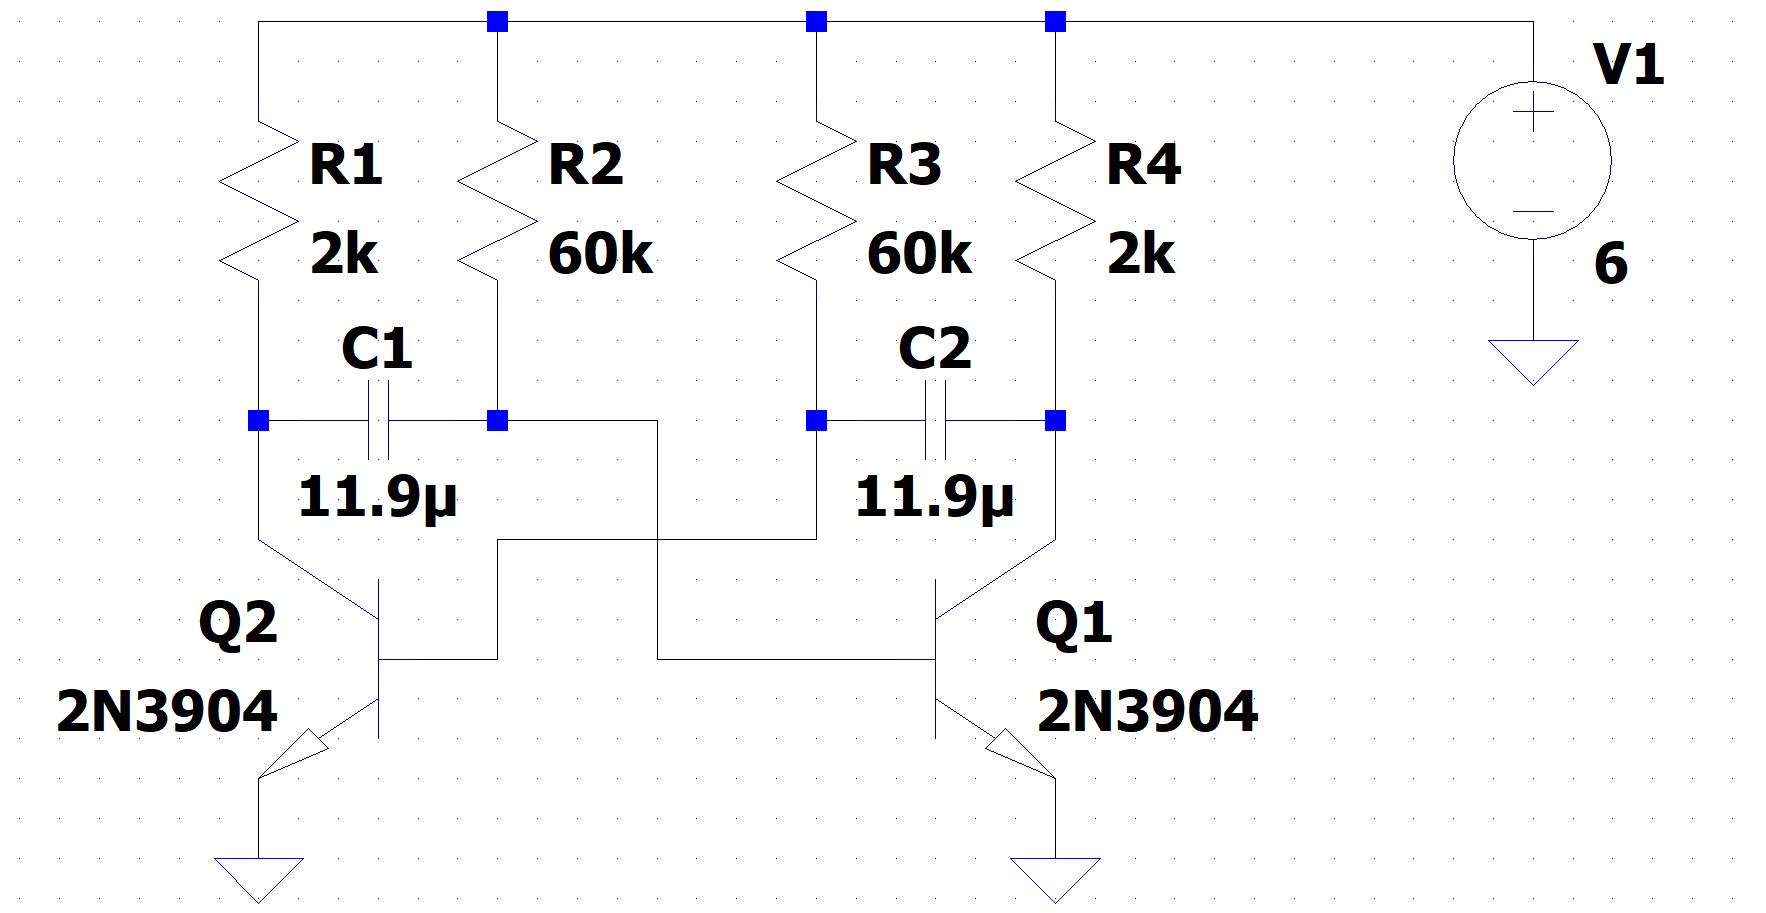
\includegraphics[width=\linewidth]{figs/мультивибр_транзисторы_схема.png}
    \caption{Схема мультивибратора на транзисторах.}
    \label{fig:мультивибр_транзисторы_схема}
\end{figure}

\begin{figure}[H]
    \centering
    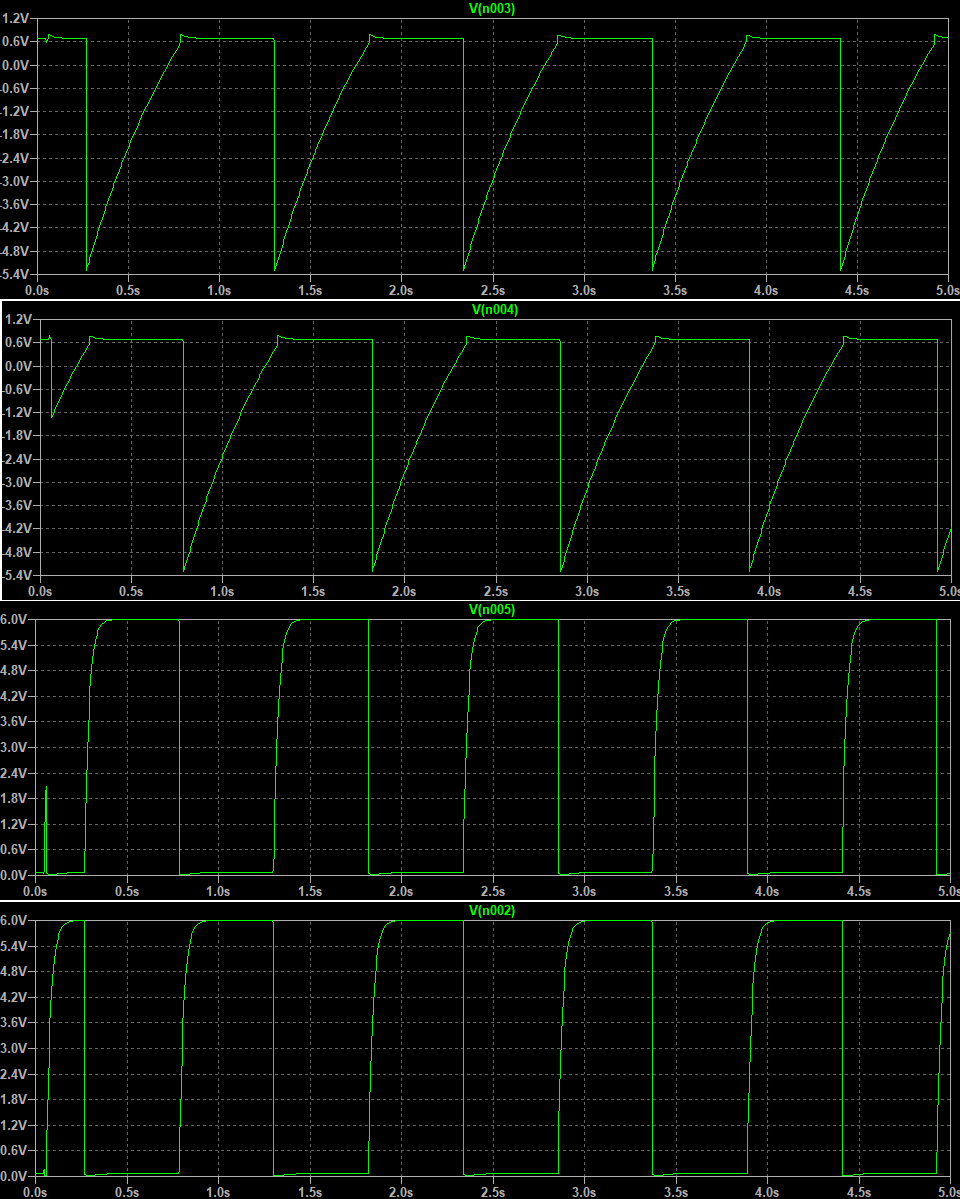
\includegraphics[width=\linewidth]{figs/Q12.png}
    \caption{Осцилограмма напряжений на базах транзисторов Q1, Q2, на
    коллекторах транзисторов Q1, Q2 соответственно.}
    \label{fig:Q12}
\end{figure}


\section*{Мультивибратор на операционном усилителе}

Соберите в LTspice схему, изображенную на рисунке \ref{fig:мультивибр_оу_схема}. Модель ОУ - AD746, диодов - 1N914.
Значения сопротивления резисторов ($R_1=R_2=60\ k\Omega$, $R_3=45\ k\Omega$, $R_4=15\ k\Omega$), 
периода повторения (50 мс) в соответствии с вариантом.
Значение емкости конденсатора рассчитаем по формуле
\begin{equation*}
    T=(R_1+R_2)C\ln(1+\frac{2R_4}{R_3})
\end{equation*}
так, чтобы период генерируемого сигнала соответствовал указанному выше.
Тогда
\begin{equation*}
    C=\frac{T}{(R_1+R_2)\ln(1+\frac{2R_4}{R_3})}\approx 8.15\cdot10^{-7}\ \text{Ф} = 0.815\ \text{мкФ}.
\end{equation*}

Осцилограммы напряжений конденсаторе и выходе схемы мультивибратора на ОУ
можно увидеть на рисунке \ref{fig:U1}. Схема успешно генерирует колебания.
Деления на осцилограмме установленны на 50 мс, и как видно,
период колебаний соответствует заданному в исходных данных.
Рассчитаем скважность:
\begin{equation*}
    Q=\frac{T}{t}=\frac{R_1+R_2}{R_1}=2. 
\end{equation*}
Данное значение отлично видно "на глаз" на осцилограмме.


\begin{figure}[H]
    \centering
    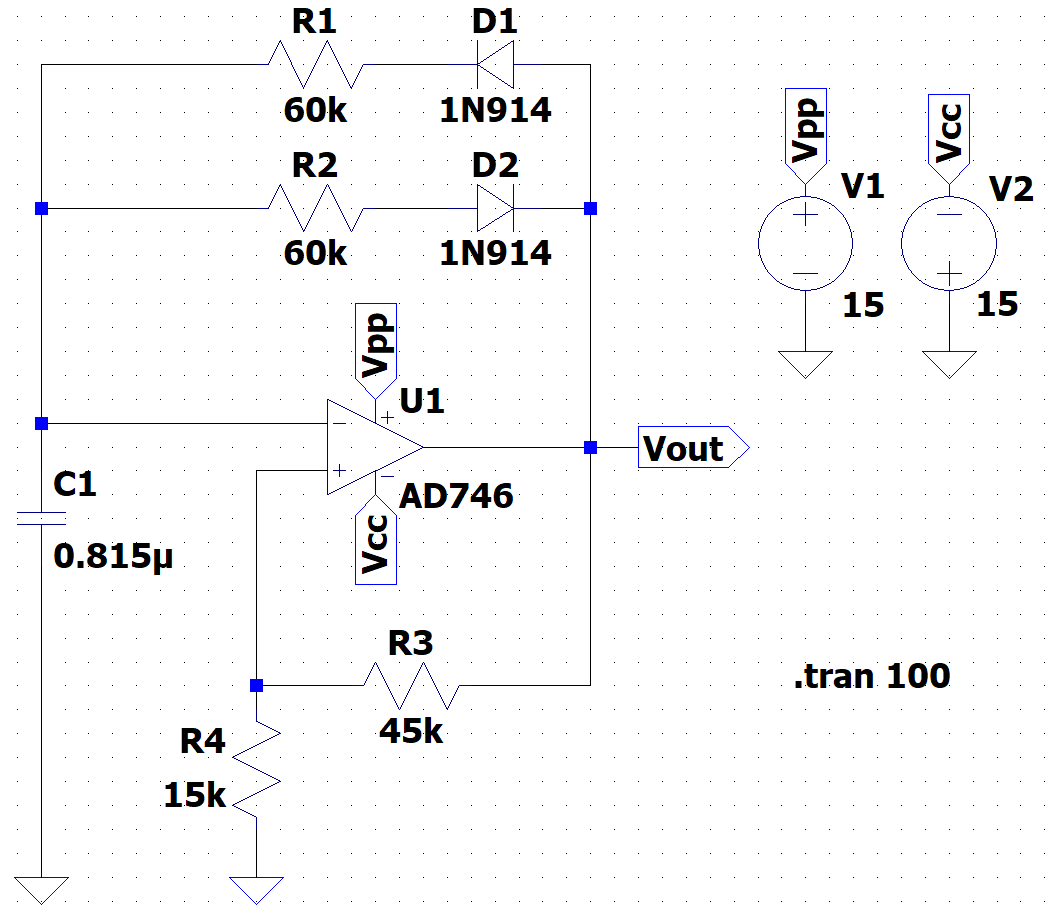
\includegraphics[width=\linewidth]{figs/мультивибр_оу_схема.png}
    \caption{Схема мультивибратора на ОУ.}
    \label{fig:мультивибр_оу_схема}
\end{figure}

\begin{figure}[H]
    \centering
    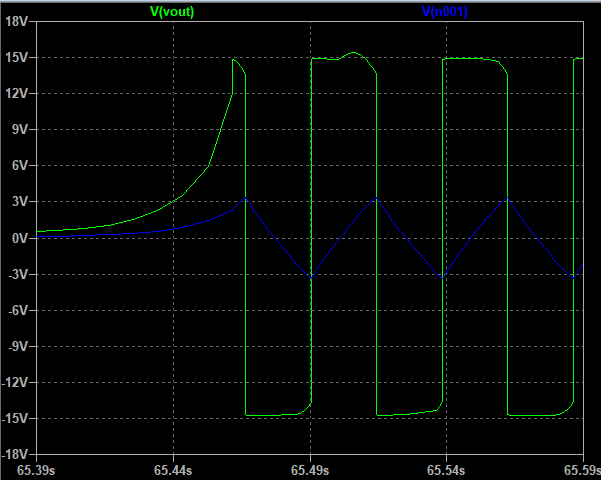
\includegraphics[width=\linewidth]{figs/U1.png}
    \caption{Осцилограмма напряжений конденсаторе и выходе схемы мультивибратора на ОУ. (зеленый график - напряжение выхода, синий - конденсатора)}
    \label{fig:U1}
\end{figure}


\section*{Заключение}

В данной лабораторной работе моделировались мультивибраторы на транзисторах и на операционном усилителе.
Были успешно сгенерированы прямоугольные колебания на обоих видах мультивибраторов.